%%%%%%%%%%%%%%%%%%%%%%%%%%%%%%%%%%%%%%%%%%%%%%%%%%%%%%%%%%%%%%%%%%
% formal-proposal-draft.tex -- ADVANCE DRAFT of the formal PhD dissertation
% proposal (document C), York/TMU Joint Graduate Program in Communication &
% Culture.
%
% NOT FOR THE ADMISSIONS APPLICATION. The formal proposal is prepared after
% admission, in consultation with the supervisor, and submitted within five
% months of passing the Qualifying Examination (Dissertation Regulations,
% rev. May 2016). It must name the supervisor and supervisory committee, and
% the program's ethics form is submitted with it. Those names are left as
% placeholders here and must not be filled in until confirmed.
%
% Structure follows the program-specific format in that document, in order:
% Title; Introduction; Objectives (problem/questions, theoretical perspective,
% expected contribution and originality); Methods and Sources (methods,
% sources, anticipated problems of access); Relationship to existing
% literature or professional practice; Proposed chapter outline; Proposed
% time line; Select Bibliography (theoretical works relevant to methodology;
% works bearing on the substance of the topic).
% Length: 8-10 pages + bibliography, maximum 3,500 words.
%
% 2026-10-20: body text is shared with proposal-rebecca.tex through
% sections/*.tex (one canonical narrative). Deliberate differences: no
% related-work table here (prose in Section 4 instead); Sources and the York
% section order are specific to this file. See revision_audit.md.
%
% The two-part Select Bibliography is generated from references.bib into
% formal-proposal-bibliography.tex (see the comment at the top of that file).
% Compiles with pdfLaTeX, XeLaTeX or LuaLaTeX. No BibTeX run is needed.
%%%%%%%%%%%%%%%%%%%%%%%%%%%%%%%%%%%%%%%%%%%%%%%%%%%%%%%%%%%%%%%%%%
\documentclass[letterpaper,12pt]{article}
\usepackage{iftex}
\ifPDFTeX
  \usepackage[T1]{fontenc}
  \usepackage[utf8]{inputenc}
  \usepackage{mathptmx}
\else
  \usepackage{fontspec}
  \setmainfont{texgyretermes}[Extension=.otf, UprightFont=*-regular,
    BoldFont=*-bold, ItalicFont=*-italic, BoldItalicFont=*-bolditalic]
\fi
\usepackage[top=25mm, bottom=25mm, left=25mm, right=25mm]{geometry}
\usepackage{setspace}
\usepackage{enumitem}
\usepackage{needspace}
\usepackage{booktabs}
\usepackage{tabularx}
\usepackage{tikz}
\usetikzlibrary{arrows.meta, positioning, fit, backgrounds}
\usepackage[font=small, labelfont=bf]{caption}
\usepackage[round,authoryear]{natbib}
\usepackage{xurl}
\usepackage[hidelinks]{hyperref}

\setlength{\parindent}{0pt}
\setlength{\parskip}{6pt}
\setlength{\emergencystretch}{1.5em}
\setlist{itemsep=2pt, topsep=4pt, parsep=0pt}
\onehalfspacing
\widowpenalty=10000
\clubpenalty=10000

\begin{document}

\begin{center}
  {\bf\Large Whose Contribution Counts?}\\[4pt]
  {\bf\large Generative AI, Cultural Participation and Collective Authorship in Research-Creation}\\[12pt]
  {\bf Roman Jahandideh}\\[3pt]
  PhD Dissertation Proposal (research-creation option)\\
  Joint Graduate Program in Communication \& Culture, York University\\[3pt]
  Supervisor: [to be confirmed]\quad Supervisory committee: [to be confirmed]\\[3pt]
  \textit{Advance draft prepared before admission; not an approved proposal.}
\end{center}

\section*{Summary}
% sections/summary.tex -- shared abstract/summary.
% \input by proposal-rebecca.tex (Summary) and formal-proposal-draft.tex
% (non-technical Summary required by the Dissertation Regulations).
% Edit here once; both documents change. No sectioning commands in this file.
I am an artistic practitioner and researcher working through
research-creation. Trained in architecture and landscape architecture, I build
interactive 3D environments and multiplayer games and study them with
participants. This project asks how generative artificial intelligence
(GenAI), meaning the models, interfaces and platforms that operate them,
reorganizes interpretive authority and collective authorship in
collaborative artistic practice. Three subquestions follow: how selected
tools, defaults and facilitation arrangements amplify, standardize, misread
or pass over participants' culturally situated contributions; how
collaborators negotiate uptake, refusal, credit and responsibility among
themselves, the group, the artist-facilitator, models, platforms and
institutions; and how artistic methods and a public artwork can make these
usually hidden distributions perceptible, debatable and revisable. As
platforms mediate more cultural production, they help decide whose meanings
become legible and who answers for shared work. The design begins with my own studio inquiry, followed by
consultation with four to six practitioners, workshops with 18--24 adult
interdisciplinary artists in three cohorts with participant observation,
semi-structured focus groups, and the co-creation of a room-scale
collaborative installation proposed for exhibition at York University. It
would contribute a communication-and-culture account of how GenAI
redistributes interpretive authority, a research-creation method for
studying it, and an artwork that keeps those negotiations visible.


\section{Introduction}
% sections/problem.tex -- problem and wider cultural stakes (shared).
% B: "The problem and its wider stakes"; C: "Introduction".
% Claims and sources: source_verification.md, section E.
GenAI systems increasingly mediate access to and participation in some forms
of cultural production. Their training data, defaults, moderation rules,
access conditions and contractual terms are shaped largely by platform
companies \citep{crawford2021}. I therefore treat GenAI not as a neutral
tool or autonomous artist, but as part of a cultural infrastructure that
includes interfaces, institutions, facilitators and unequal conditions of
access.

Three mechanisms give this infrastructure social stakes. The first is \emph{platformized interpretive
authority}. \citet[276]{richards2025} argues that the ``safe and helpful''
assistant functions ``as a proxy for authority''; Caines found that
subscription tiers, privacy conditions and opacity shaped what she and her
students could make \citep[187--188, 194]{caines2026steaming}; and Caines
and Watson describe a project whose outcome lay ``completely in the hands of
the corporations that designed the software''
\citep[267]{caines2023consultation}. The second is \emph{cultural
legibility}: models may privilege, flatten, standardize, mistranslate,
misrecognize or pass over culturally situated expression. South Asian
participants found that text-to-image models reproduced an outsider's gaze
on their cultures \citep{qadri2023}, and AI writing suggestions moved Indian
writers toward Western styles \citep{agarwal2025}; each finding concerns
particular models and tasks. The third is the gap between
\emph{technical provenance and social authorship}: a system can record who
supplied what while collaborators credit someone else, and artists' work has
entered training data without their consent \citep{jiang2023}.
Environmental cost, labour displacement and misinformation form the wider
context \citep[182]{caines2026steaming} but are not objects of this study.

Participation and authorship matter because they determine who takes part
in meaning-making, whose contribution remains recognizable, who can revise
or refuse a model's transformation, who receives public credit and who is
held responsible when collaborative work circulates. They are where platform
power becomes practical in everyday cultural production. One qualitative
study cannot explain AI's effect on society, but situated research-creation
can make these processes observable and yield analytically transferable
concepts.


\section{Objectives}

\subsection{Research problem and questions}
% sections/questions.tex -- research questions, provisional argument and terms (shared).
\textbf{Central question.} How do GenAI systems reorganize interpretive
authority and collective authorship in collaborative artistic practice?

\begin{enumerate}[label=\textbf{SQ\arabic*.}, leftmargin=*]
  \item \emph{Translation and cultural legibility.} How do selected models,
        interfaces, defaults, moderation systems and facilitation
        arrangements privilege, amplify, flatten, standardize, mistranslate,
        misrecognize, refuse or pass over participants' self-identified and
        culturally situated contributions? (Studio records; episodes;
        transformation histories; platform documentation.)
  \item \emph{Negotiation and governance.} How do collaborators negotiate
        uptake, revision, refusal, attribution, credit, responsibility and
        collective decisions among contributors, the group, the
        artist-facilitator, models, platforms and institutions? (Field
        notes; group rules; version histories; focus groups.)
  \item \emph{Research-creation and public form.} How can collaborative
        artistic methods and the form of a public artwork materialize
        otherwise hidden distributions of interpretive authority and leave
        them open to debate and revision? (Scores; versions of the work;
        studio journal.)
\end{enumerate}

The exhibition is a creative, analytical and dissemination outcome. Because
audience data will not be collected, the study will not make empirical
claims about audience reception.

\textbf{Provisional argument.} GenAI does not merely add a nonhuman
collaborator to collective art-making; it may reorganize the conditions
under which contributions become visible, legible, transformable,
contestable, attributable, creditable, ownable and accountable. The research
may confirm, complicate or reject this proposition, and it treats refusal,
silence, failure, non-use, withdrawal, disagreement and unresolved parallel
versions as meaningful outcomes.

\textbf{Terms.} \emph{Participation} means taking part in consequential
decisions, not merely receiving access to or interacting with a system.
\emph{Recognition} concerns whether a contribution remains perceptible and
attributable within the shared work. \emph{Interpretive authority} is the
capacity to influence or decide what a contribution means, how it is
transformed and what it becomes. \emph{Attribution} or \emph{credit} is the
public acknowledgement of a contribution. \emph{Authorship} is a socially
and institutionally negotiated claim that a person or group substantively
shaped the work. \emph{Ownership} is a legal or contractual claim.
\emph{Responsibility} concerns who is expected to answer for the work and
its consequences. \emph{Technical provenance} is a system's record of
inputs, transformations or versions: evidence, but not a definitive record
of social authorship, cultural recognition or responsibility.
\emph{Culturally situated contributions} include languages, references,
idioms, memories, aesthetic conventions, performance practices and forms of
community knowledge that participants themselves identify as significant.
The project will not judge cultural authenticity or treat anyone as
representing a culture or community.


\subsection{Theoretical perspective}
% sections/framework.tex -- theoretical framework (shared).
% Claims and sources: source_verification.md, section E.
\textbf{Participation as power.} Jenkins and colleagues describe
participatory cultures as ones in which ``members believe their
contributions matter'' \citep[3]{jenkins2006}. \citet{carpentier2016} asks whether participants
share power at the moments when decisions are made, which separates
participation from access and interaction. Discussing
\emph{Artificial Hells} \citep{bishop2012}, Bishop warns that ``there is no
point celebrating an `ethical' working process as a goal in itself''
\citep[176]{eschenburg2014}.

\textbf{Mediation and infrastructure.} \citet{suchman2007} shows that agency
is figured and attributed in situated practice. AI-mediated communication research describes models that modify
messages between people \citep{hancock2020}, and the companies that run them
present themselves as ``platforms'' while shaping the terms by which they are
judged \citep{gillespie2010}.

\textbf{Collective production and recognition.} Becker's sociology of art
worlds treats art as the work of many cooperating actors and activities, not
the named artist alone (\citealp{becker1982}, as discussed by
\citealp[39--46]{parker2014}). \citet[32]{hodson2019} shows that even
when design is opened to others, ``the story is still told in terms of
design-led collaboration''.

\textbf{Research-creation and critical improvisation.} Research-creation
makes the making a way of knowing \citep{chapman2012} and can challenge the
norms of the fields it crosses (\citealp[37]{loveless2019}, quoted in
\citealp[255]{caines2023consultation}). As discussed by Caines and Watson, drawing on
Caines's ``Fragile Devices'' \citep{caines2021fragile}, improvisation is a
method built on ``real-time decision-making with others, surprise, supported
and accountable risk taking, deep listening, and \ldots{} the reconfiguration
of mistake'' \citep[273]{caines2023consultation}. Caines also reads her GenAI work as ``a kind of
critical improvisation practice'' marked by ``a constant cycle of navigating
power, adaptation, surprise, failure, and creation''
\citep[193]{caines2026steaming}. I ask how that cycle unfolds when the
material is one another's offers.


\subsection{Expected contribution and originality}
% sections/contributions.tex -- contributions at five levels (shared).
Without presuming its findings, the study aims to contribute a conceptual
account of how GenAI mediation redistributes interpretive authority,
recognition and responsibility in collective art-making; situated empirical
evidence of how collaborators negotiate transformations, defaults, refusals
and credit; a research-creation method combining studio inquiry,
participant observation, focus groups, episode and version analysis and
public co-creation; a collaborative installation and scores that keep these
negotiations perceptible; and situated principles for consent, refusal,
attribution, accessibility, platform choice and shared governance rather
than universal rules. Its originality lies not in new software but in
following the same contributions across studio, workshop, focus group and
exhibition.


\section{Methods and sources}

\subsection{Research methods}
% sections/design.tex -- research-creation design, phases and participants (shared).
% Claims and sources: source_verification.md, sections A and E.
The project follows the program's research-creation option: a substantial
creative work and a 150--200-page written dissertation that carries the
theoretical argument \citep{comcult_rc}. Its five phases overlap and feed
back into one another (Figure~\ref{fig:overview}).

\textbf{Phase 1: Studio inquiry and tool ecology.} Before any participants
are involved, I will undertake a sustained period of my own artistic
research into collaboration and GenAI. I will select three or four tool
families, for example text, image, voice or audio, and spatial media
integrated through Unity, against explicit criteria: artistic relevance,
cost and access, data and privacy terms, whether inputs and outputs can be
documented, degree of user control, known cultural defaults and feasibility.
Where quality allows, one will be a locally run open-weight model, and
non-AI processes stay in the ecology. The phase produces experiments, scores,
a failure log, a reflexive journal and preliminary works, and reads
interface documentation, terms of service and model cards as cultural
documents. It asks how each tool structures prompting, refusal and
authorship; it is not software benchmarking.

\textbf{Phase 2: Consultation and pilots.} Four to six adult artists,
improvisers, facilitators or creative technologists will act as advisors in
pilot sessions that refine scores, access provisions, tool choices and
consent and credit protocols. They are not main participants, and I will
call them co-researchers only if they share decisions and credit.

\textbf{Phase 3: Collaborative workshops.} The provisional sample is 18--24
adults in three cohorts of six to eight: artists, performers and
improvisers, designers, creative technologists and community-engaged arts
practitioners. Open calls to arts communities in Toronto and York Region and
to AMPD networks, excluding anyone I teach, will seek variation in
discipline, GenAI experience, adult age and cultural and linguistic
background; the sample is not representative. I begin with adults because
the work is public, consent and authorship are complex to negotiate, and the
platforms' data practices are contested. Six to eight people can make work
together and be observed closely; three cohorts allow cross-case comparison. The scale rests on information power, meaning a
specific sample, an established framework and repeated, dense encounters
\citep{malterud2016}, not on statistical power or declared saturation
\citep{braun2021saturate}.

Each cohort will attend four connected workshops of about two and a half
hours. The sequence, set after Phases 1 and 2, will include: agreeing
group conventions and making together without assuming AI is needed; experiments with more than one form of GenAI mediation and with
AI/non-AI combinations; repeated chances to accept, revise, reroute, refuse,
remove or reinterpret outputs; collective rules for attribution, data use,
credit, reuse and decisions; reflection on misreading, standardization,
surprise, exclusion and productive failure; and movement toward materials
and scores for the final artwork. I will conduct disclosed participant
observation with field notes and the reflexive journal. With consent, I will
collect recordings, prompts and outputs, version histories, logs, artifacts
and group-authored rules. A log records system events, not intentions.

\textbf{Phase 4: Focus groups.} Each cohort will then join one
semi-structured focus group of 60--90 minutes on voice, recognition,
cultural legibility, the authority of models and platforms, ownership,
responsibility, refusal, access and desired changes. Focus groups make
participants' interaction part of the data \citep{kitzinger1994}. Short
individual follow-ups are offered only to those who need a private way to
discuss disagreement or power.

\textbf{Phase 5: Co-creation and exhibition.} The workshops lead toward a
large collaborative artwork proposed for the first-floor Art Gallery at
York's Markham Campus, which has shown creative-technologies exhibitions
\citep{yorkmarkham2024}, subject to supervisory, venue, resource, ethics and
participant approval. Its form (projection, spatial sound, interactive 3D
media, performance or installation) will emerge from the workshops. It
should make the research perceptible, not illustrate findings, for instance
by exposing traces of rejection, model defaults and contested credit. Participants decide whether and
how their material, names, voices and images appear; consent to exhibit is
separate from consent to research, and no audience data will be collected.
For examination, the work will be documented through installation records,
executable media where feasible, scores, process records and an annotated
account of its iterations.


\begin{figure}[ht]
\centering
\setstretch{1.0}
% figures/study-overview.tex -- research-creation design schematic (TikZ).
% Redesigned 2026-10-20: replaces the earlier technical pipeline diagram.
% Included by proposal-rebecca.tex and by figures/study-overview-standalone.tex.
% Requires: \usetikzlibrary{arrows.meta, positioning, fit, backgrounds}
% Fixed font sizes so the figure renders identically in 11pt and 12pt documents.
% Grayscale-safe: meaning is carried by position, line style and labels.
%   solid arrows  = sequence of phases
%   dashed arrows = feedback that revises earlier decisions
%   dotted arrows = evidence moving into interpretation
%   grey bands    = processes that run across every phase
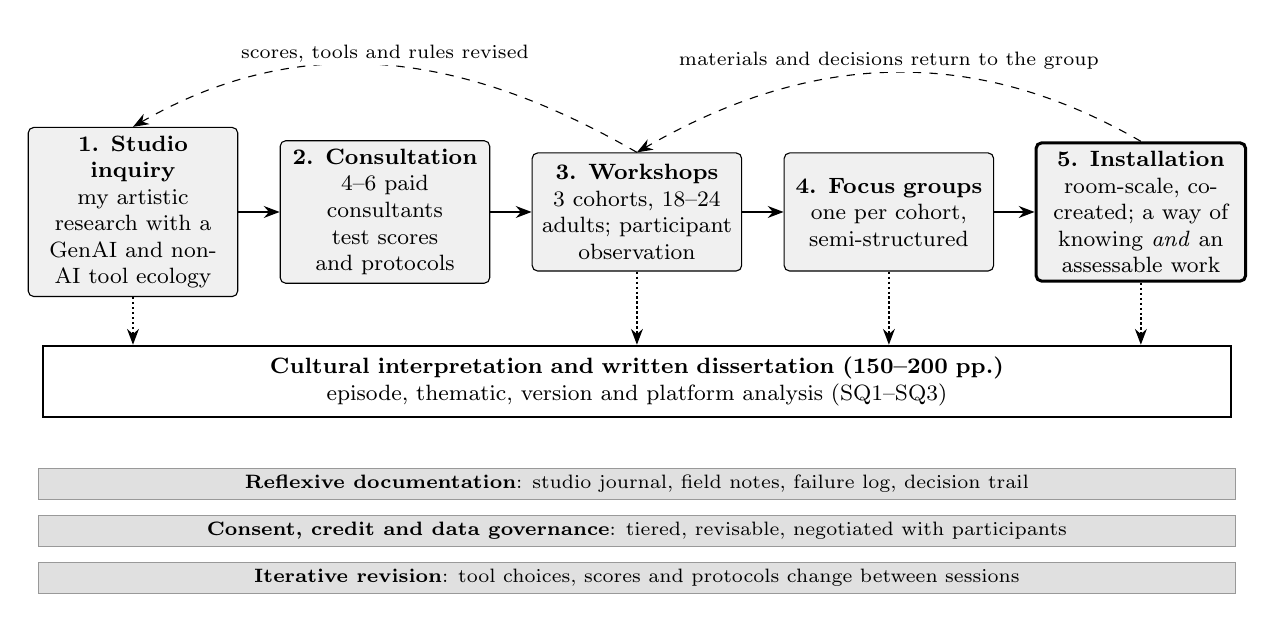
\begin{tikzpicture}[
  font=\fontsize{8}{9.6}\selectfont,
  >={Stealth[length=2mm]},
  every node/.append style={execute at begin node={\hyphenpenalty=10000}},
  phase/.style={draw, rounded corners=2pt, fill=black!6, align=center,
                text width=2.45cm, inner sep=3pt, minimum height=15mm},
  flow/.style={->, thick},
  back/.style={->, dashed},
  evid/.style={->, densely dotted, thick},
  lab/.style={font=\fontsize{7}{8.4}\selectfont, fill=white, inner sep=1pt},
  band/.style={draw=black!40, fill=black!12, align=center, inner sep=2.5pt,
               minimum width=15.2cm, font=\fontsize{7.5}{9}\selectfont}
]
% ---- phases ----
\node[phase] (p1) at (0,0)     {\textbf{1. Studio inquiry}\\my artistic research with a GenAI and non-AI tool ecology};
\node[phase] (p2) at (3.2,0)   {\textbf{2. Consultation}\\4--6 paid consultants test scores and protocols};
\node[phase] (p3) at (6.4,0)   {\textbf{3. Workshops}\\3 cohorts, 18--24 adults; participant observation};
\node[phase] (p4) at (9.6,0)   {\textbf{4. Focus groups}\\one per cohort, semi-structured};
\node[phase, line width=1.1pt] (p5) at (12.8,0) {\textbf{5. Installation}\\room-scale, co-created; a way of knowing \emph{and} an assessable work};
\draw[flow] (p1) -- (p2);
\draw[flow] (p2) -- (p3);
\draw[flow] (p3) -- (p4);
\draw[flow] (p4) -- (p5);
% ---- feedback ----
\draw[back] (p3.north) to[out=150, in=30] node[lab, above] {scores, tools and rules revised} (p1.north);
\draw[back] (p5.north) to[out=150, in=30] node[lab, above] {materials and decisions return to the group} (p3.north);
% ---- interpretation ----
\node[draw, thick, fill=white, align=center, text width=14.8cm, inner sep=4pt]
  (diss) at (6.4,-2.15) {\textbf{Cultural interpretation and written dissertation (150--200 pp.)}\\
  episode, thematic, version and platform analysis (SQ1--SQ3)};
\foreach \p in {p1,p3,p4,p5} \draw[evid] (\p.south) -- (\p.south |- diss.north);
% ---- cross-cutting processes ----
\node[band] (b1) at (6.4,-3.45) {\textbf{Reflexive documentation}: studio journal, field notes, failure log, decision trail};
\node[band] (b2) at (6.4,-4.05) {\textbf{Consent, credit and data governance}: tiered, revisable, negotiated with participants};
\node[band] (b3) at (6.4,-4.65) {\textbf{Iterative revision}: tool choices, scores and protocols change between sessions};
\end{tikzpicture}

\caption{Proposed research-creation design. Solid arrows show the sequence
of phases, dashed arrows feedback, and dotted arrows evidence moving into
interpretation; grey bands run across every phase.}
\label{fig:overview}
\end{figure}

% sections/analysis.tex -- analysis aligned with the subquestions (shared).
Analysis is aligned with the subquestions. For SQ1, I will analyse selected
workshop episodes multimodally, adapting the video microethnography
\citet{mcarthur2015} used for interface interaction, and read interfaces,
terms of service and model documentation as cultural documents. For SQ2,
reflexive thematic analysis of the focus groups \citep{braun2019} is read
alongside field notes, episodes and group-created rules. For SQ3, version
analysis charts each state of the work against the contributors who shaped
it, after the version timelines of \citet[10]{hodson2019}. A system log records events, inputs and
transformations; it does not independently establish intention, authorship,
recognition or responsibility. Contribution trajectories will therefore be
interpreted through participant accounts, negotiated attribution, contextual
observation, material versions and acknowledged uncertainty, not used as a
surveillance record. Discrepant cases, including refusal and non-use,
reflexive memos and a decision trail keep the interpretation accountable. Because models cannot be isolated from
facilitation, platform, group history or changing tool versions, claims will
be situated and analytically transferable rather than causal.


% sections/ethics.tex -- ethics, governance, accessibility (shared).
Consent will be tiered and revisable \citep{strengers2021}, given separately
for recording, model input, research analysis, exhibition, documentation and
reuse. Every activity has a manual route, and participants may decline
particular forms of visibility. No identifiable voice, image or text, and no
culturally sensitive material, will be sent to a model without specific
consent. Participants will be told that commercial services may retain or
reuse prompts and outputs, and I will prefer local or institutionally
approved tools where feasible. Groups will agree in advance how withdrawal works once material has
been remixed: identifiable contributions are removed where feasible, but a
remixed contribution cannot always be fully separated from exhibited work.
Legal ownership, contractual terms, public credit, felt authorship, research
authorship and responsibility are treated as distinct. Data will be
minimized, stored securely with restricted access, and retained and deleted
on a documented schedule. Participants and consultants will receive
honoraria and access costs; if funding is inadequate, I will reduce the
sample or the number of sessions rather than rely on unpaid artistic labour.
Alternatives to sound-only or vision-only interaction, and
help at every level of AI literacy, support different forms of
participation. Participants will not
be asked to disclose or perform trauma, to represent a community, or to
educate me about cultural misrecognition. Participation alone does not make
the process equitable \citep{birhane2022}.


\subsection{Sources}
Primary sources are those generated in the five phases described above,
together with interface documentation, terms of service and model cards.
Secondary sources are discussed in Section~\ref{sec:lit}.

\subsection{Anticipated problems of access}
% sections/access.tex -- anticipated problems of access (shared).
% C: "Anticipated problems of access"; B: closing paragraph of the ethics section.
Three problems of access are foreseeable. \emph{Participants:} recruitment
depends on open calls; if a cohort cannot complete the series, its completed
sessions remain usable as a smaller case and a replacement cohort will be
considered. \emph{Venue:} the Markham Campus gallery is a proposal, not a
commitment; if it is unavailable, the work will be presented in another
campus space or as a documented installation for examination.
\emph{Tools:} platforms may close, change terms or prices, or update models
during the study, so Phase 1 keeps substitutes, including a local model, and
records each tool's version as part of the evidence.


\section{Relationship to existing literature and professional practice}\label{sec:lit}
% sections/position.tex -- artistic-practitioner position (shared).
% Facts from the author's CV and publications only; see source_verification.md, F.
I come to this question as a practitioner. Architecture at Tabriz Islamic
Art University and landscape architecture at Istanbul Technical University
taught me to treat designed environments as media of social life:
thresholds, paths and light shape who gathers, who is seen and how people
move together. In ITU's Virtual Landscape Lab I studied how people perceive
mediated environments \citep{jahandideh2023}. My current master's in
Interactive Arts and Technology at Simon Fraser University, in Steve
DiPaola's iViz Lab, moved this practice into interactive 3D and game
environments: I build multiplayer worlds and physiological interfaces in
Unity and C\#, use image-generation models in design work, and study these
systems with participants. One study is accepted at ACM ISS 2026
\citep{jahandideh_teammate_ms}; another is under revision
\citep{jahandideh_bioterrarium_ms}. The through-line runs from designing
spaces, to designing mediated environments, to asking who controls how a
technical system represents and translates people: in the teammate study,
participants accepted a shared heart-rate cue only if they controlled who saw
it. As artist, system designer, facilitator, participant observer and analyst,
I will hold power over what participants can do and how their actions are
read, so documenting my own decisions is part of the method.


% sections/artists.tex -- artistic field and precedents (shared).
% Each work checked against the artist's or venue's own page; source_verification.md, D.
Four artistic practices inspire the project's questions, and each changes a
specific decision in its design. Anna Ridler's
\emph{Myriad (Tulips)} exhibits thousands of tulip photographs she labelled
by hand, making a dataset's labour and classification into the artwork
\citep{ridler2018}; it leads me to keep prompts, labels and rejected outputs
as exhibitable material. Stephanie Dinkins's \emph{Not the Only One} is
trained on oral histories from three generations of women in her family and
hosted locally to protect community data \citep{dinkins_ntoo}; it makes data
custody a criterion for choosing tools. Holly Herndon and Mat Dryhurst's
\emph{The Call} trained choral models on recordings of fifteen community
choirs and tested a data trust \citep{herndon2024call}; because its
governance was designed by the artists and institution, my workshops
instead ask participants to set credit and data rules. Sougwen Chung's
\emph{Drawing Operations} pairs her drawing with robotic systems trained on
her own drawings and gestures \citep{chung_dou}, a model of improvised
co-performance that my scores extend to many contributors. Caines's \emph{multiPLAY}, with workshops, open studios and an
artist hackathon for Canadian improvisers \citep{multiplay}, and
\emph{ImprovEnabled}, a strengths-based improvisation project developed with
community partners \citep{improvenabled}, are methodological precedents for
community-engaged improvisation, supported risk, listening and accessible
workshop design; they are not research sites for this study.


% sections/fit.tex -- program and supervisor fit (shared).
% Program wording checked 2026-10-20; source_verification.md, section A.
The project belongs to Technology in Practice because it examines critically
how GenAI platforms, interfaces and institutions configure cultural practice,
and to Media \& Culture because it studies cultural production,
representation, participation, authorship and labour. It answers the
program's aim of ``promoting the application of critical theory and
research'' \citep{york_overview} and its PhD objectives, which name
``creative exhibitions'' among the routes to independent research
\citep{york_phdpage}. Dr.\ Caines's work on critical improvisation, socially
responsive creative technologies and GenAI is its closest ground; her GenAI
study focused mostly on course and workshop design
\citep[176]{caines2026steaming}, whereas this project follows how
collaborators negotiate one another's contributions in sustained art-making
and public exhibition.


\section{Proposed chapter outline}

\begin{enumerate}[label=\arabic*., leftmargin=*, itemsep=0pt]
  \item GenAI and cultural participation.
  \item Participation, mediation and collective production.
  \item Methodology: research-creation, studio, workshops and reflexivity.
  \item The studio inquiry and the tool ecology as cultural document.
  \item Translation, recognition and refusal in the workshops.
  \item Credit, responsibility and the public artwork.
  \item Protocols and wider stakes.
\end{enumerate}

\section{Proposed timeline}

Dates assume full-time study from Fall 2027.

\begin{description}[font=\normalfont, labelwidth=8.9em, leftmargin=9.5em,
  labelsep=0.6em, itemsep=0pt]
  \item[Jan--Apr 2029] Proposal approval; ethics application; Phase 1 studio
        inquiry continues.
  \item[May--Aug 2029] Phase 2 consultations and pilots.
  \item[Sep 2029--Apr 2030] Phase 3 workshops with three cohorts; Phase 4
        focus groups.
  \item[May--Dec 2030] Phase 5 co-creation and proposed exhibition; analysis.
  \item[Jan--Jun 2031] Writing and revision of chapters.
  \item[Jul--Aug 2031] Submission and defence (Year 5 in reserve).
\end{description}

%TC:ignore
% formal-proposal-bibliography.tex -- GENERATED; do not edit by hand.
% Two-part Select Bibliography required by the program's proposal format:
% (1) theoretical works relevant to the methodology, (2) works bearing on the
% substance of the topic. Entries are plainnat output from references.bib,
% limited to works cited in formal-proposal-draft.tex.
\providecommand{\natexlab}[1]{#1}
\providecommand{\url}[1]{\texttt{#1}}
\expandafter\ifx\csname urlstyle\endcsname\relax
  \providecommand{\doi}[1]{doi: #1}\else
  \providecommand{\doi}{doi: \begingroup \urlstyle{rm}\Url}\fi
\section*{Select bibliography}
\renewcommand{\bibsection}{\subsection*{\refname}}
\renewcommand{\refname}{Theoretical and methodological works}
\begin{thebibliography}{19}

\bibitem[Becker(1982)]{becker1982}
Howard~S. Becker.
\newblock \emph{Art Worlds}.
\newblock University of California Press, Berkeley, 1982.

\bibitem[Birhane et~al.(2022)Birhane, Isaac, Prabhakaran, Diaz, Elish, Gabriel,
  and Mohamed]{birhane2022}
Abeba Birhane, William Isaac, Vinodkumar Prabhakaran, Mark Diaz,
  Madeleine~Clare Elish, Iason Gabriel, and Shakir Mohamed.
\newblock Power to the people? {O}pportunities and challenges for participatory
  {AI}.
\newblock In \emph{Equity and Access in Algorithms, Mechanisms, and
  Optimization (EAAMO '22)}, pages 1--8, 2022.
\newblock \doi{10.1145/3551624.3555290}.

\bibitem[Bishop(2012)]{bishop2012}
Claire Bishop.
\newblock \emph{Artificial Hells: Participatory Art and the Politics of
  Spectatorship}.
\newblock Verso, London, 2012.

\bibitem[Braun and Clarke(2019)]{braun2019}
Virginia Braun and Victoria Clarke.
\newblock Reflecting on reflexive thematic analysis.
\newblock \emph{Qualitative Research in Sport, Exercise and Health},
  11\penalty0 (4):\penalty0 589--597, 2019.
\newblock \doi{10.1080/2159676X.2019.1628806}.

\bibitem[Braun and Clarke(2021)]{braun2021saturate}
Virginia Braun and Victoria Clarke.
\newblock To saturate or not to saturate? {Questioning} data saturation as a
  useful concept for thematic analysis and sample-size rationales.
\newblock \emph{Qualitative Research in Sport, Exercise and Health},
  13\penalty0 (2):\penalty0 201--216, 2021.
\newblock \doi{10.1080/2159676X.2019.1704846}.

\bibitem[Caines(2021)]{caines2021fragile}
Rebecca Caines.
\newblock Fragile devices: Improvisation as an interdisciplinary research
  methodology.
\newblock In Michael Bull and Marcel Cobussen, editors, \emph{The Bloomsbury
  Handbook of Sonic Methodologies}, pages 325--340. Bloomsbury Academic, New
  York, 2021.
\newblock \doi{10.5040/9781501338786.ch-019}.

\bibitem[Carpentier(2016)]{carpentier2016}
Nico Carpentier.
\newblock Beyond the ladder of participation: An analytical toolkit for the
  critical analysis of participatory media processes.
\newblock \emph{Javnost -- The Public}, 23\penalty0 (1):\penalty0 70--88, 2016.
\newblock \doi{10.1080/13183222.2016.1149760}.

\bibitem[Chapman and Sawchuk(2012)]{chapman2012}
Owen Chapman and Kim Sawchuk.
\newblock Research-creation: Intervention, analysis and ``family
  resemblances''.
\newblock \emph{Canadian Journal of Communication}, 37\penalty0 (1):\penalty0
  5--26, 2012.
\newblock \doi{10.22230/cjc.2012v37n1a2489}.

\bibitem[Eschenburg(2014)]{eschenburg2014}
Madeline Eschenburg.
\newblock Artificial hells: A conversation with {Claire Bishop}.
\newblock \emph{Contemporaneity: Historical Presence in Visual Culture},
  3:\penalty0 174--178, 2014.
\newblock \doi{10.5195/contemp.2014.113}.

\bibitem[Gillespie(2010)]{gillespie2010}
Tarleton Gillespie.
\newblock The politics of `platforms'.
\newblock \emph{New Media \& Society}, 12\penalty0 (3):\penalty0 347--364,
  2010.
\newblock \doi{10.1177/1461444809342738}.

\bibitem[Hancock et~al.(2020)Hancock, Naaman, and Levy]{hancock2020}
Jeffrey~T. Hancock, Mor Naaman, and Karen Levy.
\newblock {AI}-mediated communication: Definition, research agenda, and ethical
  considerations.
\newblock \emph{Journal of Computer-Mediated Communication}, 25\penalty0
  (1):\penalty0 89--100, 2020.
\newblock \doi{10.1093/jcmc/zmz022}.

\bibitem[Jenkins et~al.(2006)Jenkins, Clinton, Purushotma, Robison, and
  Weigel]{jenkins2006}
Henry Jenkins, Katie Clinton, Ravi Purushotma, Alice~J. Robison, and Margaret
  Weigel.
\newblock Confronting the challenges of participatory culture: Media education
  for the 21st century.
\newblock Occasional paper on digital media and learning, John D. and Catherine
  T. MacArthur Foundation, 2006.
\newblock URL
  \url{https://www.macfound.org/media/article_pdfs/jenkins_white_paper.pdf}.

\bibitem[Kitzinger(1994)]{kitzinger1994}
Jenny Kitzinger.
\newblock The methodology of focus groups: The importance of interaction
  between research participants.
\newblock \emph{Sociology of Health \& Illness}, 16\penalty0 (1):\penalty0
  103--121, 1994.
\newblock \doi{10.1111/1467-9566.ep11347023}.

\bibitem[Loveless(2019)]{loveless2019}
Natalie Loveless.
\newblock \emph{How to Make Art at the End of the World: A Manifesto for
  Research-Creation}.
\newblock Duke University Press, Durham, NC, 2019.
\newblock \doi{10.1215/9781478004646}.

\bibitem[Malterud et~al.(2016)Malterud, Siersma, and Guassora]{malterud2016}
Kirsti Malterud, Volkert~Dirk Siersma, and Ann~Dorrit Guassora.
\newblock Sample size in qualitative interview studies: Guided by information
  power.
\newblock \emph{Qualitative Health Research}, 26\penalty0 (13):\penalty0
  1753--1760, 2016.
\newblock \doi{10.1177/1049732315617444}.

\bibitem[McArthur(2015)]{mcarthur2015}
Victoria McArthur.
\newblock \emph{Me, Myself, and Interface: The Role of Affordances in Digital
  Visual Self-Representational Practices}.
\newblock PhD thesis, York University, Graduate Programme in Communication \&
  Culture, 2015.
\newblock URL \url{http://hdl.handle.net/10315/30044}.

\bibitem[Parker(2014)]{parker2014}
Felan Parker.
\newblock \emph{Playing Games with Art: The Cultural and Aesthetic Legitimation
  of Digital Games}.
\newblock PhD thesis, York University and Ryerson University, Graduate Program
  in Communication \& Culture, 2014.
\newblock URL \url{http://hdl.handle.net/10315/28164}.

\bibitem[Strengers et~al.(2021)Strengers, Sadowski, Li, Shimshak, and
  Mueller]{strengers2021}
Yolande Strengers, Jathan Sadowski, Zhuying Li, Anna Shimshak, and
  Florian~`Floyd' Mueller.
\newblock What can {HCI} learn from sexual consent? {A} feminist process of
  embodied consent for interactions with emerging technologies.
\newblock In \emph{Proceedings of the 2021 CHI Conference on Human Factors in
  Computing Systems}, pages 1--13, 2021.
\newblock \doi{10.1145/3411764.3445107}.

\bibitem[Suchman(2007)]{suchman2007}
Lucy~A. Suchman.
\newblock \emph{Human--Machine Reconfigurations: Plans and Situated Actions}.
\newblock Cambridge University Press, Cambridge, 2 edition, 2007.
\newblock \doi{10.1017/CBO9780511808418}.

\end{thebibliography}

\renewcommand{\refname}{Works bearing on the substance of the topic}
\begin{thebibliography}{19}

\bibitem[Agarwal et~al.(2025)Agarwal, Naaman, and Vashistha]{agarwal2025}
Dhruv Agarwal, Mor Naaman, and Aditya Vashistha.
\newblock {AI} suggestions homogenize writing toward {Western} styles and
  diminish cultural nuances.
\newblock In \emph{Proceedings of the 2025 CHI Conference on Human Factors in
  Computing Systems}, pages 1--21, 2025.
\newblock \doi{10.1145/3706598.3713564}.

\bibitem[Caines(2019)]{multiplay}
Rebecca Caines.
\newblock {multiPLAY}: Exploring digital community-engagement with {Canadian}
  improvisers.
\newblock Project website. Canada Council for the Arts, with the International
  Institute for Critical Studies in Improvisation, 2019.
\newblock URL \url{https://multiplay.ca/}.
\newblock Project 2019--2021; accessed 2026-10-20.

\bibitem[Caines(2026)]{caines2026steaming}
Rebecca Caines.
\newblock {STE(AI)}ming across disciplines and into the future: Generative
  artificial intelligence for ethics, access, and interdisciplinary skills
  development in classrooms and communities.
\newblock \emph{American Journal of STEM Education: Issues and Perspectives},
  21:\penalty0 175--202, 2026.
\newblock \doi{10.32674/aztpg851}.

\bibitem[Caines and Stewart(2015)]{improvenabled}
Rebecca Caines and Michelle Stewart.
\newblock {ImprovEnabled}: Improvisation and {FASD}.
\newblock Project website, University of Regina, 2015.
\newblock URL \url{https://improvenabled.rebeccacaines.org/canada/}.
\newblock Pilot 2015--2016; accessed 2026-10-21.

\bibitem[Caines and Watson(2023)]{caines2023consultation}
Rebecca Caines and Brandon Watson.
\newblock ``{T}hat's not art, it's just consultation!'': Performing innovation
  in socially responsive creative technologies research.
\newblock \emph{Performance Matters}, 9\penalty0 (1--2):\penalty0 253--277,
  2023.
\newblock URL
  \url{https://performancematters-thejournal.com/index.php/pm/article/view/449}.

\bibitem[Chung(2014)]{chung_dou}
Sougwen Chung.
\newblock Drawing operations unit, generations {I--VII}.
\newblock Artwork series, 2014--. Artist's website, 2014.
\newblock URL \url{https://sougwen.com/work/memory-drawing-operations}.
\newblock Accessed 2026-10-20.

\bibitem[Dinkins(2018)]{dinkins_ntoo}
Stephanie Dinkins.
\newblock Not the only one.
\newblock Artwork, 2018--. Artist's project page, 2018.
\newblock URL \url{https://www.stephaniedinkins.com/ntoo.html}.
\newblock Accessed 2026-10-20.

\bibitem[Goodfellow~Craig(2026)]{yfile2026sshrc}
Ashley Goodfellow~Craig.
\newblock {SSHRC} invests \$9.3{M} in {York}-led social sciences, humanities
  research.
\newblock YFile, York University, July 2026.
\newblock URL
  \url{https://www.yorku.ca/yfile/2026/07/24/sshrc-invests-9-3m-in-york-led-social-sciences-humanities-research/}.
\newblock Published 2026-07-24; accessed 2026-10-20.

\bibitem[Herndon and Dryhurst(2024)]{herndon2024call}
Holly Herndon and Mat Dryhurst.
\newblock The call.
\newblock Exhibition, Serpentine North Gallery, London, 4 October 2024 -- 2
  February 2025, 2024.
\newblock URL
  \url{https://www.serpentinegalleries.org/whats-on/holly-herndon-mat-dryhurst-the-call/}.
\newblock Accessed 2026-10-20.

\bibitem[Hodson(2019)]{hodson2019}
Elise Hodson.
\newblock \emph{Design in Motion: The Everyday Object and the Global Division
  of Design Labour}.
\newblock PhD thesis, York University, Joint Graduate Program in Communication
  \& Culture, 2019.
\newblock URL \url{http://hdl.handle.net/10315/36271}.

\bibitem[Jahandideh(2026)]{jahandideh_bioterrarium_ms}
Roman Jahandideh.
\newblock Embedding physiological responsiveness into game world dynamics:
  Designing bio-adaptive game worlds for embodied self-regulation.
\newblock Manuscript under revision, 2026.

\bibitem[Jahandideh et~al.(2023)Jahandideh, Jahandideh, and
  Kim]{jahandideh2023}
Roman Jahandideh, Aran Jahandideh, and Ikhwan Kim.
\newblock Creating immersive virtual landscapes: A user-centered approach to
  enhance depth perception in head-mounted displays.
\newblock In \emph{Digital Design Reconsidered: Proceedings of the 41st
  Conference on Education and Research in Computer Aided Architectural Design
  in Europe (eCAADe 2023)}, volume~1, pages 149--158, 2023.
\newblock \doi{10.52842/conf.ecaade.2023.1.149}.

\bibitem[Jahandideh et~al.(2026)Jahandideh, Jahandideh, and
  DiPaola]{jahandideh_teammate_ms}
Roman Jahandideh, Aran Jahandideh, and Steve DiPaola.
\newblock Reading a remote teammate's body: A body-worn sensing interface for
  group coordination in a distributed interactive space.
\newblock In \emph{Companion Proceedings of the Conference on Interactive
  Surfaces and Spaces (ISS Companion '26)}, Turin, Italy, 2026. ACM.
\newblock Accepted; to appear.

\bibitem[Jiang et~al.(2023)Jiang, Brown, Cheng, Khan, Gupta, Workman, Hanna,
  Flowers, and Gebru]{jiang2023}
Harry~H. Jiang, Lauren Brown, Jessica Cheng, Mehtab Khan, Abhishek Gupta, Deja
  Workman, Alex Hanna, Johnathan Flowers, and Timnit Gebru.
\newblock {AI} art and its impact on artists.
\newblock In \emph{Proceedings of the 2023 AAAI/ACM Conference on AI, Ethics,
  and Society}, pages 363--374, 2023.
\newblock \doi{10.1145/3600211.3604681}.

\bibitem[{Joint Graduate Program in Communication \&
  Culture}(2021)]{comcult_rc}
{Joint Graduate Program in Communication \& Culture}.
\newblock {PhD} research-creation dissertation ({April} 2021).
\newblock York University and Toronto Metropolitan University, 2021.
\newblock URL
  \url{https://www.yorku.ca/gradstudies/cmct/wp-content/uploads/sites/327/2023/08/COMCULT_PHD-research_CREATE_April-2021-Updated.pdf}.
\newblock Accessed 2026-10-20.

\bibitem[Qadri et~al.(2023)Qadri, Shelby, Bennett, and Denton]{qadri2023}
Rida Qadri, Renee Shelby, Cynthia~L. Bennett, and Remi Denton.
\newblock {AI}'s regimes of representation: A community-centered study of
  text-to-image models in {South Asia}.
\newblock In \emph{Proceedings of the 2023 ACM Conference on Fairness,
  Accountability, and Transparency}, pages 506--517, 2023.
\newblock \doi{10.1145/3593013.3594016}.

\bibitem[Richards(2025)]{richards2025}
Grayson Richards.
\newblock \emph{Nothing to See Here: Generative {AI}, Neoliberal Crisis, and
  Intensified Counterinsurgency}.
\newblock PhD thesis, York University, Graduate Program in Communication and
  Culture, 2025.
\newblock URL \url{https://hdl.handle.net/10315/43566}.

\bibitem[Ridler(2018)]{ridler2018}
Anna Ridler.
\newblock Myriad ({Tulips}).
\newblock Artwork, 2018. Artist's project page, 2018.
\newblock URL \url{https://annaridler.com/works/myriad-tulips}.
\newblock Accessed 2026-10-20.

\bibitem[{York University Markham Campus}(2024)]{yorkmarkham2024}
{York University Markham Campus}.
\newblock {York University Markham Campus} welcomes community to first official
  open house.
\newblock York University, November 2024.
\newblock URL \url{https://www.yorku.ca/markham/?p=4174}.
\newblock Posted 2024-11-20; accessed 2026-10-20.

\end{thebibliography}

%TC:endignore

\end{document}
